\section{Preprocesamiento}

Antes de iniciar con el proceso de construcción de \textit{embeddings} y modelos de clasificación se realizó una estandarización o preprocesamiento a los datos de ambos \textit{datasets}. Est preprocesamiento se puede encontrar en el cuaderno adjunto  \texttt{preprocessing.iynb}. Se empezó por importar los diálogos de ambas series, los cuales se encontraban en formatos distintos. \\

Por un lado, para el \textit{dataset} de Los Simpsons, los datos ya se encontraban discriminados por personaje, por lo que el único trabajo que se hizo fue el de seleccionar los dialogos de los 4 personajes principales (Homero, Marge, Bart y Lisa Simpson). Por otro lado, para el \textit{dataset} de Friends, se tenían el script crudo de cada uno de los episodios. De esta manera se leyeron todos los archivos verificando su contenido en cada línea. En caso de encontrar alguno de los personajes principales (Rachel, Ross, Chandler, Monica, Joey o Phoebe) se agregaba el contenido seguido de los dos puntos \textit{(:)} y se le agregaba la etiqueta del personaje. \\

Así las cosas, se obtuvieron el siguiente número de sentencias (o frases) por cada uno de los personajes principales (véase cuadro \ref{tab:dist-datos}). En estas se observa que la distribución de las clases es similar para tres de los cuatro personajes de los Simpsons. No obstante, Homero acapara poco más del 40\% de las sentencias, lo que sugiere un desbalance considerable en el caso de este \textit{dataset}. Por el lado de la serie de Friends, se observa una distribución mucho más balanceada de las clases, con una diferencia menor al $4\%$ entre la clase con más datos y la de menos datos.

\begin{table}[H]
\caption{Distribución de las clases (número de sentencias para cada personaje) en cada uno de los \textit{datasets}.}
\label{tab:dist-datos}
\centering
\begin{minipage}{0.45\textwidth}
\centering
\begin{tabular}{|l|l|}
\hline
\textbf{Character} & \textbf{N° Sentences} \\ \hline
Homer & 27850 \\ \hline
Marge & 13172 \\ \hline
Bart & 12995 \\ \hline
Lisa & 10756 \\ \hline
\end{tabular}
\caption*{a) Simpsons }

\end{minipage}\hfill
\begin{minipage}{0.45\textwidth}
\centering
\begin{tabular}{|l|l|}
\hline
\textbf{Character} & \textbf{N° Sentences} \\ \hline
Rachel & 8506 \\ \hline
Ross & 8262 \\ \hline
Chandler & 7686 \\ \hline
Moncia & 7620 \\ \hline
Joey & 7572 \\ \hline
Phoebe & 6831 \\ \hline
\end{tabular}
\caption*{b) Friends}

\end{minipage}

\end{table}

Ahora bien, a dichas sentencias se les aplico una estandarización la cual consistió en los siguientes procesos:

\begin{itemize}
    \item lower case:
    
    \item colloquial term removal:
    
    \item simple lematization:
\end{itemize}

Una vez hecha esta estandarización se obtuvo el tamaño de las frases (número de tokens en cada sentencia) para cada uno de los \textit{datasets}.... \\

Adicionalmente, se separaron de una vez los \textit{datasets} en sets de entrenamiento (train), validación (val) y prueba (test), con una distribución de 70\%, 15\% y 15\% respectivamente. 

\begin{figure}[H]
    \centering
    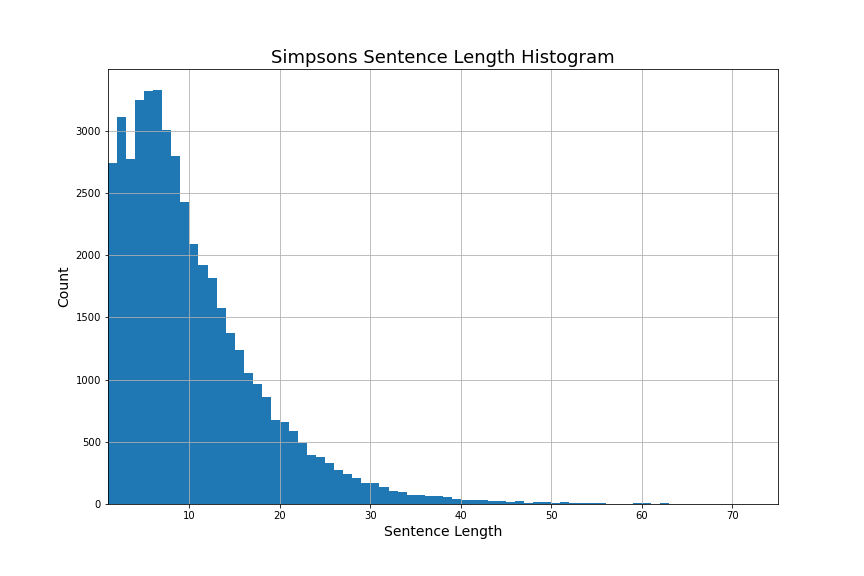
\includegraphics[width=0.8\textwidth]{results/preprocessing/simpsons_hist.png}
    \caption{Tamaño de las frases en los diálogos de los Simpsons}
    \label{fig:simpsons_hist}
\end{figure}



\begin{figure}[H]
    \centering
    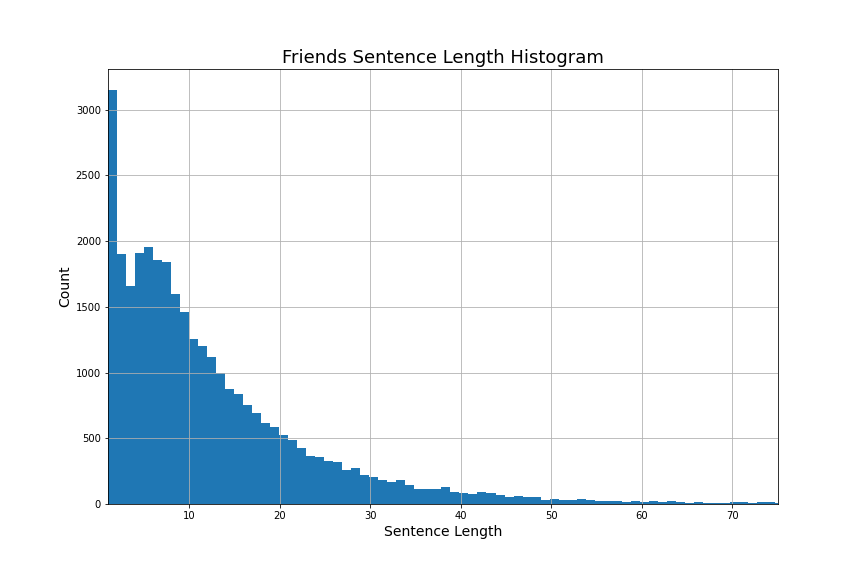
\includegraphics[width=0.8\textwidth]{results/preprocessing/friends_hist.png}
    \caption{Tamaño de las frases en los diálogos de Friends}
    \label{fig:friends_hist}
\end{figure}